\documentclass[journal,10pt,twoside, a4paper]{IEEEtran}
\usepackage{cite,graphicx,array,color,amssymb,balance}
\usepackage[cmex10]{amsmath}


\title{Machine learning aided DSP in optical coherent receivers}

\author{
    \IEEEauthorblockN{L.H.P. Driessen\\}
    \IEEEauthorblockA{l.h.p.driessen@student.tue.nl, ID 0962549}
}
\begin{document}
\maketitle

\begin{abstract}
    A recurrent neural network has been used as a substitution to parts of the DSP chain in optical coherent receivers. Results with simulated data show that this technique not yet comparable to conventional filtering techniques. An accuracy of 98.5952\% (BER of $\mathbf{1.408\cdot 10^{-2}}$) has been achieved in simulated QPSK data with an SNR of 15 and a transmission differential group delay of 40ps. In real, frequency-offset compensated, 8-QAM data, an accuracy of 83.2145\% (BER of $\mathbf{1,67855\cdot 10^{-1}}$) has been achieved.
\end{abstract}

\section{Introduction}
\IEEEPARstart{F}{iber-optic} communication has replaced lots of the electrical communication in the last decades due to its lower interference and higher bandwidth. Conventionally, direct-detection with on-off keying was used in optical communication. However, it is possible to achieve a greater bandwidth by using a coherent communication system\cite{coherent_detection,DSP_beyond}. Latest developments in coherent optical transmission have shown data communication rates in the Tb/s range\cite{coherent_detection, DSP_beyond, dsp+ml}.

Coherent optical fiber communication was studied in the 1980s. The main advantage over direct-detection was the ability to transmit data over longer distances\cite{coherent_detection}. In the 1990s and the beginning of the 2000s, research on coherent detection decreased due to the advent of wavelength division multiplexing (WDM). Research on coherent systems continued in 2005, which showed promising results\cite{continue}. The main advantage of coherent systems is that it benefits not only from light intensity, but also utilizes information such as light polarization and phase. This makes it suitable to deploy higher order modulations like QPSK and QAM, which results in higher data rates. These modulations come at the cost of higher complexity. It requires extra hardware to convert the signal to the electrical domain, as detection of polarization and phase of light is not feasible to do in the optical domain\cite{coherent_detection}. Digital signal processing (DSP) is used to recover the polarization, intensity and phase of the signal. Also, signal impairments due to channel imperfections can be compensated by DSP\cite{coherent_detection, DSP_2, DSP_beyond}. Some of these impairments, like polarization mode dispersion (PMD), are stochastic\cite{nonlinear} and have so far been compensated by linear filters.

A different approach to recover received optical signals might be to aid the DSP with machine learning methods. This is because machine learning techniques can to be useful in solving complex statistical problems. Different parts in the receiver could be substituted by these techniques to enhance the DSP performance. In this paper, the proof of concept of machine learning aided DSP in optical coherent receivers is provided and its feasibility is analyzed.

\section{Fiber-optic coherent communication}
The overall system structure in optical coherent communication is depicted schematically in Fig.~\ref{fig:coherent_detection}. The transmitter subsystem is colored blue and the receiver part red. An optical fiber is placed between the two subsystems. The use of multiple wavelengths (WDM) is omitted as this does not affect the general structure of both transmitter and receiver. The transmitter, medium and receiver are discussed next. After that, the DSP part of the receiver is addressed separately.

\begin{figure}
    \centering
    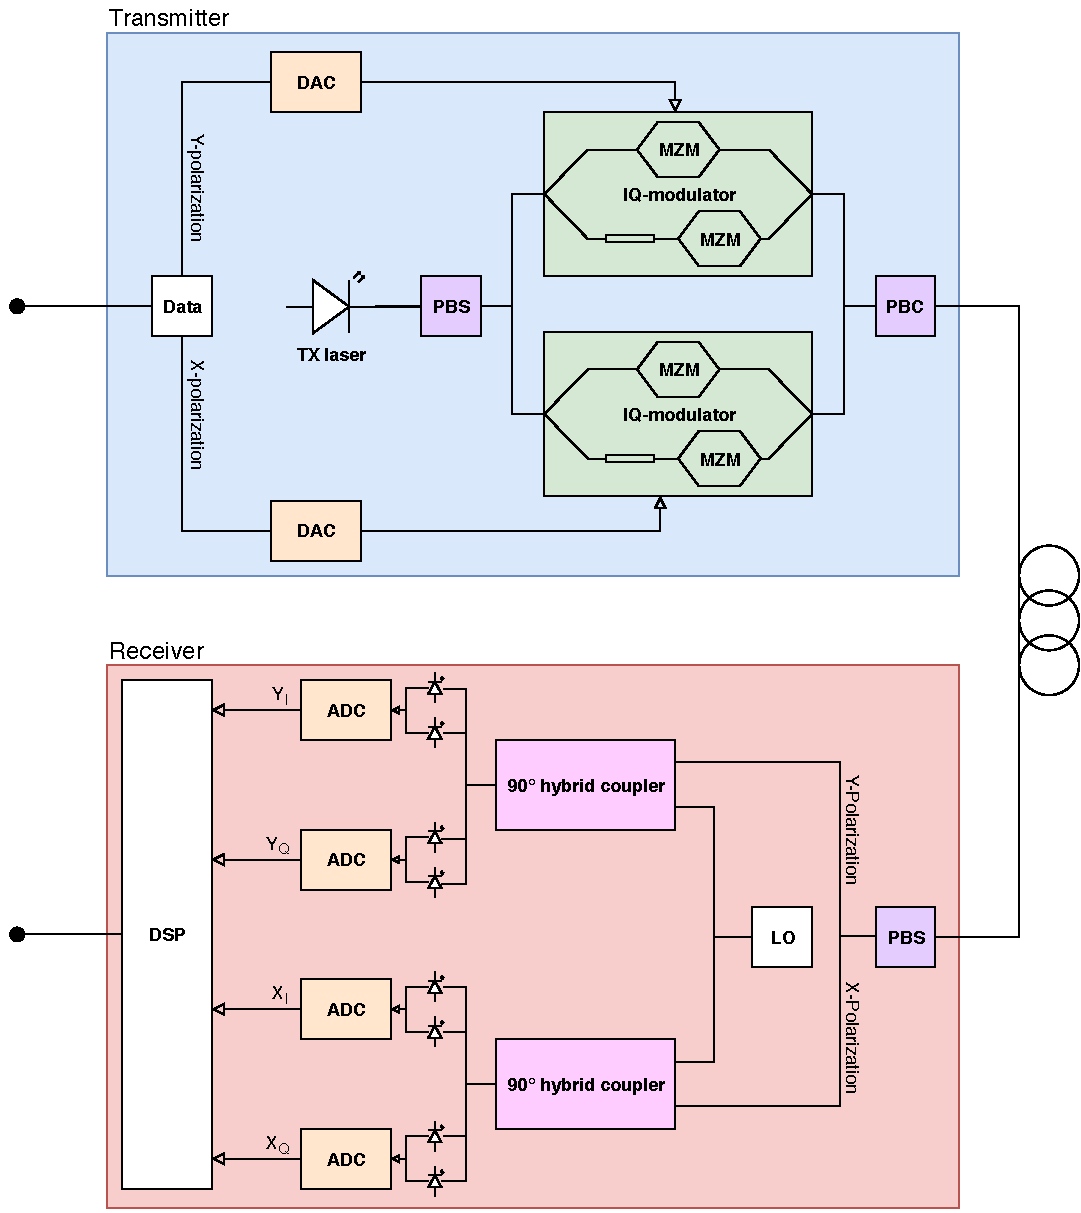
\includegraphics[width=0.9\linewidth]{images/coherent_detection}
    \caption{Schematic representation of an optical coherent detection system}
    \label{fig:coherent_detection}
\end{figure}

\subsection{Transmitter}
The transmitter in an optical coherent system consists of a continuous wave (CW) laser with a small spectral linewidth. This laser is sent through a polarizing beam splitter (PBS), which splits the incoming light into two orthogonal linear polarized beams. 

The two beams are fed into in-phase and quadrature (IQ) modulators, which main function is to encode data onto the linear polarized beam. This data first goes through a digital to analog converter (DAC) and is sent into the IQ modulators. These IQ modulator are realized by substrates of $LiNbO_3$ or $InP$, which change their refractive indices linearly depending on the applied voltage. This effect is called the Pockels effect. This IQ modulator consists of two Mach-Zehnder Modulators (MZM) in a Push-Pull configuration. This configuration exhibits an amplitude modulating behaviour. Having two MZMs which are phase-shifted by 90 degrees results in an in-phase and quadrature amplitude modulator.

The two IQ modulated orthogonal polarized beams are combined in the polarizing beam combiner (PBC) into an elliptical polarized beam. All required data information is incorporated in this beam. Then, the beam is sent through the optical fiber.

\subsection{Medium}\label{ch:Medium}
When travelling through the glass fiber, the signal is distorted. Due to group velocity dispersion (GVD) the duration of optical pulses changes. This is a result of the varying propagation velocities of wavelets within a group of wavelengths that is sent through the fiber. Also, Gaussian white noise is added to the signal as a result of quantum-mechanical vacuum fluctuations\cite{coherent_detection}. These effects are polarization independent. 

Besides polarization independent impairments, there also exist impairments that depend on the polarization. PMD is an effect that occurs because of random imperfections in the optical fiber. Asymmetrical properties and other imperfections cause the two polarizations to travel at a slightly different speed. This results in a temporal difference between the two polarizations when the signal is received\cite{PMD}. This is proportional to the square root of the distance of the medium. Related is the polarization dependent loss (PDL), which is energy losses that are different for the two polarizations.

Furthermore, the two polarizations are randomly mixed with each other due to the birefringent properties of the medium\cite{coherent_detection,PMD}.

The impairments discussed so far are linear effects. The Kerr effect is an example of a non-linear effect that happens on the transmitted signal. In this effect, the transmitted energy squared is proportional to the refractive index of the fiber.

\subsection{Receiver}
The distorted signal is received and sent through a PBS. Both polarizations are mixed with a local oscillator (LO) in a 90 degree hybrid coupler. The output ports are detected by four balanced photosensitive diodes pairs. The electrical output signals of the diode pairs represent both the in-phase and quadrature energy levels for both polarizations. Retrieving 90 degree phase shifted energy levels makes sure that no phase information is lost (phase-diversity). This is done for both polarizations (polarization-diversity), which makes sure that no polarization information is lost.

Finally, the in-phase and quadrature signals for both polarizations are converted to the digital domain by analog to digital converters (ADC) and are taken care of in the electrical domain by the DSP.

\subsection{DSP}
Until now, no information has been lost in the process of converting the optical signal into the digital electrical domain. The function of the DSP in the receiver is to recover the original data by equalizing out the impairments and finding carrier and clock phase information. How the DSP works normally is depicted in Fig.~\ref{fig:dsp}.

\begin{figure}
    \centering
    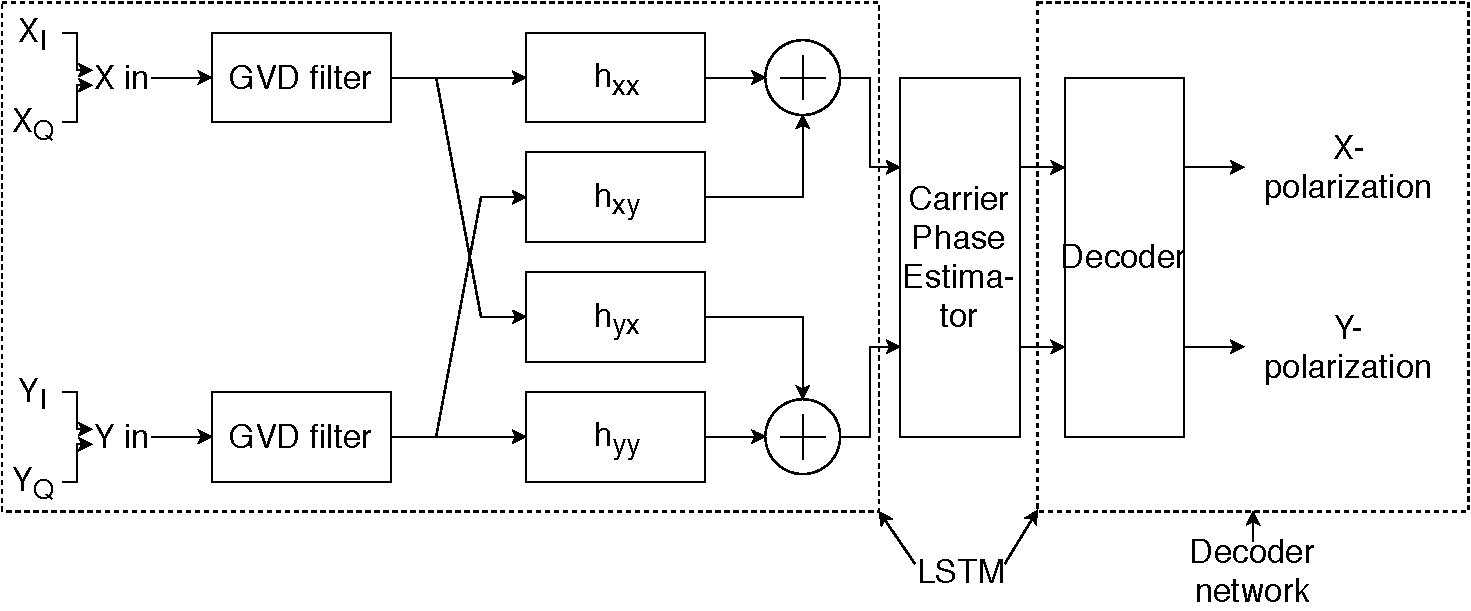
\includegraphics[width=0.9\linewidth]{Thesis/images/DSP.pdf}
    \caption{DSP chain in optical coherent receiver. The \textcircled{$+$} operator is vectorial addition}
    \label{fig:dsp}
\end{figure}

First, GVD is compensated for with a fixed filter (GVD filter). Then, all other linear impairments are compensated in a structure called butterfly structured finite impulse response (FIR) filters ($\vec{h_{xx}}$, $\vec{h_{xy}}$, $\vec{h_{yx}}$, $\vec{h_{yy}}$). These filters are adaptive since compensated impairments like PMD vary quickly over time and are stochastic. The filter tap weight algorithm used can exploit the property that incoming signals have a constant energy level. However, this Constant Modulus Algorithm (CMA) is only possible in modulation schemes with constant modulus, like M-ary PSK. The decision-directed least mean squared (DD-LMS) algorithm can be deployed on modulation schemes with varying complex moduli. This algorithm updates the filter tap weights based on the error difference between the latest estimation and the actual received bit. This algorithm works by a training sequence of symbols and providing the correct symbols to the receiver side such that it can learn how the weights of the filter taps should be set. The equations of the algorithm look as follows:
\begin{align}
    \vec{h_{xx}}(n+1) &= \vec{h_{xx}}(n) + \mu \vec{e_{X}}(n)\vec{E_x}(n), \label{dd-lms}\\
    \vec{h_{xy}}(n+1) &= \vec{h_{xy}}(n) + \mu \vec{e_{X}}(n)\vec{E_y}(n),\\
    \vec{h_{yx}}(n+1) &= \vec{h_{yx}}(n) + \mu \vec{e_{Y}}(n)\vec{E_x}(n),\\
    \vec{h_{yy}}(n+1) &= \vec{h_{yy}}(n) + \mu \vec{e_{Y}}(n)\vec{E_y}(n), \label{dd-lms2}
\end{align}
where $n$ is the symbol iteration number, $\mu$ is the step-size, $\vec{e_{X}}$ and $\vec{e_{Y}}$ are the error signals, and $\vec{E_x}$ and $\vec{E_y}$ are the energies of all the included past symbols. $\vec{e_{X}}$ and $\vec{e_{Y}}$ are defined to be the difference between the energy of respectively the in-phase and quadrature signal components and the expected in-phase and quadrature components, which are provided in training mode.

Afterwards, the carrier phase is recovered (Carrier phase estimator). This can be done with the M-th viterbi-viterbi algorithm\cite{coherent_detection,viterbi}, which retrieves the unwanted residue carrier phase offset. Alternatively, a single stage\cite{1stagebps} or two-stage\cite{2stagebps} blind phase search (BPS) algorithm can be used. After carrier phase compensation, the signal can finally be decoded and all information can be extracted (Decoder).

\section{Machine learning techniques}
%The concept of machine learning is that an computational algorithm is formed, which is not explicitly programmed, but is rather incrementally formed with the use of data. This data is called the training data and it improves the current algorithm in small steps using the principles of statistics. Because machine learning is based on statistics and not on predefined behaviour, machine learning can be seen as a black box solution.


%\subsection{Artificial neural networks}
Within machine learning, artificial neural networks are commonly used to develop algorithmic solutions. An example of an artificial neural network is given in Fig.~\ref{fig:nn}. In the example network, the input values, $\vec{x}_i$ for $i\in \{1..4\}$ are multiplied with edge weights that are incorporated in a weight matrix $\mathbf{W}^{(1)}$. A bias vector $\vec{b}^{(1)}$ is added to the result. To keep the elements in this vector within certain bounds and to add non-linearity, the vector is first sent through an activation function. A commonly used activation function is the Sigmoid function $\sigma(x) = \frac{1}{1+e^{-x}}$. The elements of the resulting vector are the nodes of the first hidden layer in the neural network, $\vec{a}_j^{(2)}$ for $j\in \{1..6\}$. Mathematically, the next layer $\vec{a}^{(n+1)}$ is calculated by 
\begin{equation}
    \vec{a}^{(n+1)} = \sigma\left(\vec{a}^{(n)}\mathbf{W}^{(n)}+\vec{b}^{(n)}\right),
\end{equation}
where $n$ is a layer number. To account for the first and last layer, $\vec{a}^{(1)} = \vec{x}$ is the input layer, and $\vec{a}^{(m)} = \vec{h}$ is the output layer, where $m$ is the amount of hidden layers in the network + 2.

The output values are compared with the correct labels with a loss-function. Based on the chosen loss-function, the network weights and biases are adapted to more suitable values through a operation called backpropagation\cite{backpropagation}, which closely resembles the DD-LMS algorithm from equations \ref{dd-lms}-\ref{dd-lms2}.

\begin{figure}
    \centering
    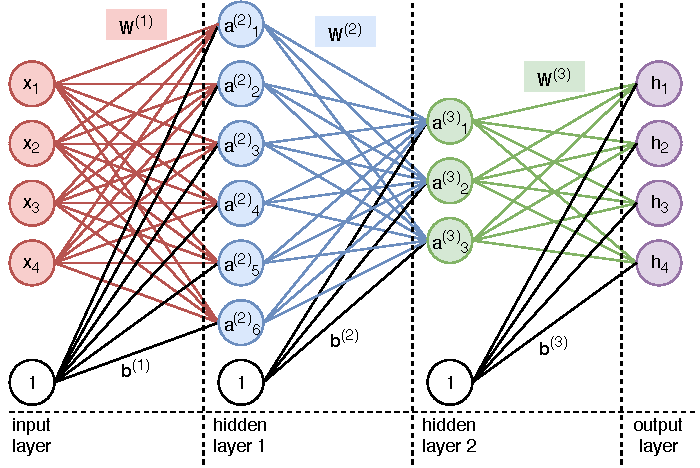
\includegraphics[width=0.9\linewidth]{Thesis/images/nn.pdf}
    \caption{Example of artificial neural network}
    \label{fig:nn}
\end{figure}

\subsection{Recurrent neural networks}
A special class of neural networks are recurrent neural networks (RNN). These networks differ from normal neural networks because the previous output is included in the new input. Thus, old or intermediate predictions are combined in the input layer of the next iteration. RNNs are most suitable when the input data has sequential behaviour.

However, RNNs have learning problems when the network has to remember data from the past that is too far away due to the vanishing/exploding gradient problem\cite{lstm}. This problem was solved in 1997 by a network structure called the Long Short Term Memory (LSTM)\cite{lstm} neural network, which is a special version of an RNN. A schematic of this type of network is shown in Fig.~\ref{fig:lstm}.

\begin{figure}
    \centering
    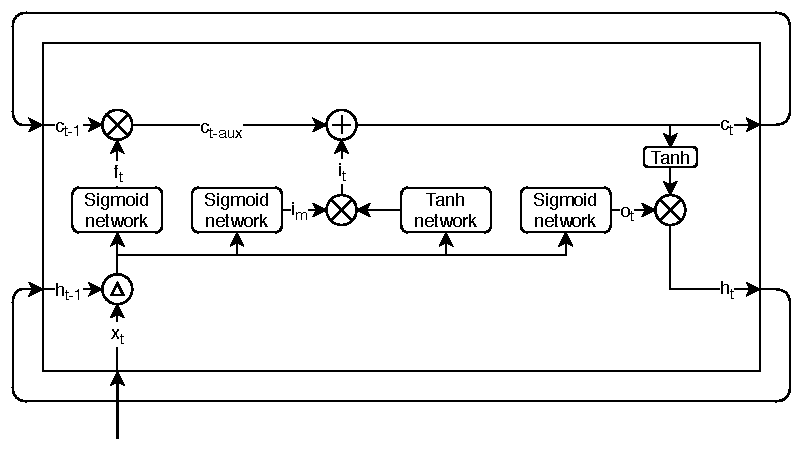
\includegraphics[width=0.9\linewidth]{Thesis/images/lstm.pdf}
    \caption{Schematic depiction of an LSTM. The \textcircled{$\scriptstyle \Delta$} operator is the concatination of the new input with the old output. The \textcircled{$+$} operator is vectorial addition. The \textcircled{$\times$} operator is elementwise multiplication between vectors.}
    \label{fig:lstm}
\end{figure}

The network has an internal state $\vec{c_t}$ which holds remembered information from the past. In every iteration, part of $\vec{c_t}$ is forgotten, added, and outputted, depending on the new input $\vec{x_t}$ and previous output $\vec{h_{t-1}}$. First, information is forgotten by element-wise multiplying $\vec{c_t}$ with a forget vector $\vec{f_t}$. This is shown in equation \ref{c_intermediate}. This vector $\vec{f_t}$ consists of values between 0 and 1: a 0 indicating to forget information, and a 1 indicating to remember information. This vector $\vec{f_t}$ is generated by a network with a Sigmoid activation function. This is shown in equation \ref{forget}. Then, new information is added to $\vec{c_t}$. To do this, the input is fed through a network with a $tanh(x) = \frac{e^x - e^{-x}}{e^x + e^{-x}}$ activation function. This information is modulated by a vector $\vec{i_m}$ from another Sigmoid driven network as shown in equation \ref{input}. The modulated vector $\vec{i_t}$ is stated in equation \ref{input_mod}. In equation \ref{new_c} it is shown how the internal state is updated. The output $\vec{h_t}$ is modulated by the vector $\vec{o_t}$, which again is the result of a Sigmoid driven network and is shown in equation \ref{output}. The final output $\vec{h_t}$ is the result of the tanh of the internal state, $tanh(\vec{c_t})$, modulated by $\vec{o_t}$. This is shown in equation \ref{new_h}. 

\begin{align}
    \vec{c_{t_{aux}}} &= \vec{f_t} \circ \vec{c_{t-1}} \label{c_intermediate}\\
    \vec{f_t} &= \sigma\left(\mathbf{W_f}\vec{x_t} + \mathbf{U_f}\vec{h_{t-1}}+\vec{b_f}\right) \label{forget}\\
    \vec{i_m} &= \sigma\left(\mathbf{W_m}\vec{x_t} + \mathbf{U_m}\vec{h_{t-1}}+\vec{b_m}\right) \label{input}\\
    \vec{i_t} &= \vec{i_m} \circ \tanh\left(\mathbf{W_i}\vec{x_t} + \mathbf{U_i}\vec{h_{t-1}}+\vec{b_i}\right) \label{input_mod}\\
    \vec{c_t} &= \vec{c_{t_{aux}}} + \vec{i_t} \label{new_c}\\
    \vec{o_t} &= \sigma\left(\mathbf{W_o}\vec{x_t} + \mathbf{U_o}\vec{h_{t-1}}+\vec{b_o}\right) \label{output}\\
    \vec{h_t} &= \vec{o_t} \circ \tanh\left(\vec{c_t}\right) \label{new_h}
\end{align}

In equations \ref{c_intermediate}-\ref{new_h}, the $t$ subscript denotes the LSTM iteration. $\mathbf{W}$ and $\mathbf{U}$ respectively denote the weight matrix for the new input $\vec{x_t}$ and the old output $\vec{h_{t-1}}$. $\vec{b}$ is the network bias. Subscripts $f$, $i$, $m$ and $o$ respectively mean "forget", "input", "modulation" and "output". The operator $\circ$ is the elementwise multiplication between vectors.

Training an LSTM happens by processing a discrete sequence of length $L$ of input data. Entries in this sequence iterate through the LSTM until it reaches the prediction of the last entry. This last prediction is compared with the correct value in a loss function and the weights and biases are updated through backpropagation. 

\section{Environment of experiment}
To experiment with the unique combination of optical fiber communication and LSTMs, an environment was created as depicted in Fig.~\ref{fig:combi}. The two used frameworks are QAMpy and PyTorch: QAMpy to generate pseudo-random complex symbols and to artificially impair them, and PyTorch to implement the recovery network.

In the LSTM experiment, the output of the QAMpy are the original symbols and the impaired symbols, which are converted in respectively an 3D and 4D tensor. This first tensor contains per batch a 2D tensor consisting of the final correct bit predictions. The second tensor contains per batch a 3D tensor: a sequence of impaired signal energy levels.

\begin{figure}
    \centering
    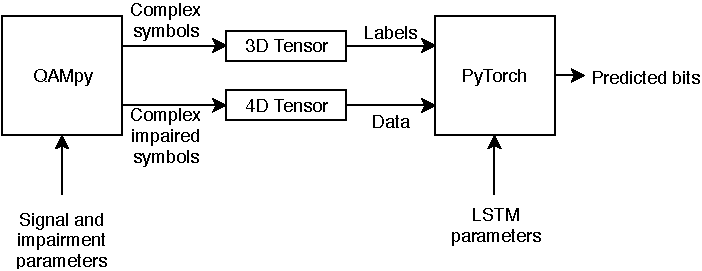
\includegraphics[width=0.9\linewidth]{Thesis/images/framework_combi.pdf}
    \caption{Environment of the conducted experiment}
    \label{fig:combi}
\end{figure}

The virtual environment can be regarded as shown in Fig.~\ref{fig:coherent_detection}, in which is indicated which parts are implemented by which framework.

\section{Experiment}
In this section, the simulated experiment is described. First, only the decoder was substituted in simulation by a regular neural network (Fig.~\ref{fig:dsp}, Decoder network). Secondly, the entire DSP chain except the carrier phase estimator was substituted in simulation by an LSTM (Fig.~\ref{fig:dsp}, LSTM). Finally, the LSTM experiment is conducted on real data. 

\subsection{Neural network decoder}
To first test if machine learning can be used in the optical receiver, the decoder has been substituted with a regular neural network. The rest of the DSP chain remains the same. A schematic depiction of the DSP chain substitution is shown in Fig.~\ref{fig:dsp} (Decoder network). For this experiment, only Gaussian noise has been added. The parameters of the simulation are shown in Table~\ref{tab:linear}.

\begin{table}
    \centering
    \caption{Parameters of data and neural network in decoder experiment}
    \label{tab:linear}
    \begin{tabular}{c|c}
        Parameter & Value\\
        \hline
        Modulation scheme & 64-QAM\\
        Generated symbols per polarization & $2^{20}$\\
        SNR & 15\\
        Hidden nodes & 32 (1 layer)\\
        Activation function & ReLU\\
        Batch size & 64\\
        Learning rate & 0.001\\
        Loss function & Cross entropy\\
        Training batches/Testing batches ratio & 75\%/25\%\\
    \end{tabular}
\end{table}

The results are shown in Fig.~\ref{fig:linear}. The different colors show how the decision boundaries of the network look like in the constellation plot. After training, the final achieved accuracy using the test data was 99.9886\%.

\begin{figure}
    \centering
    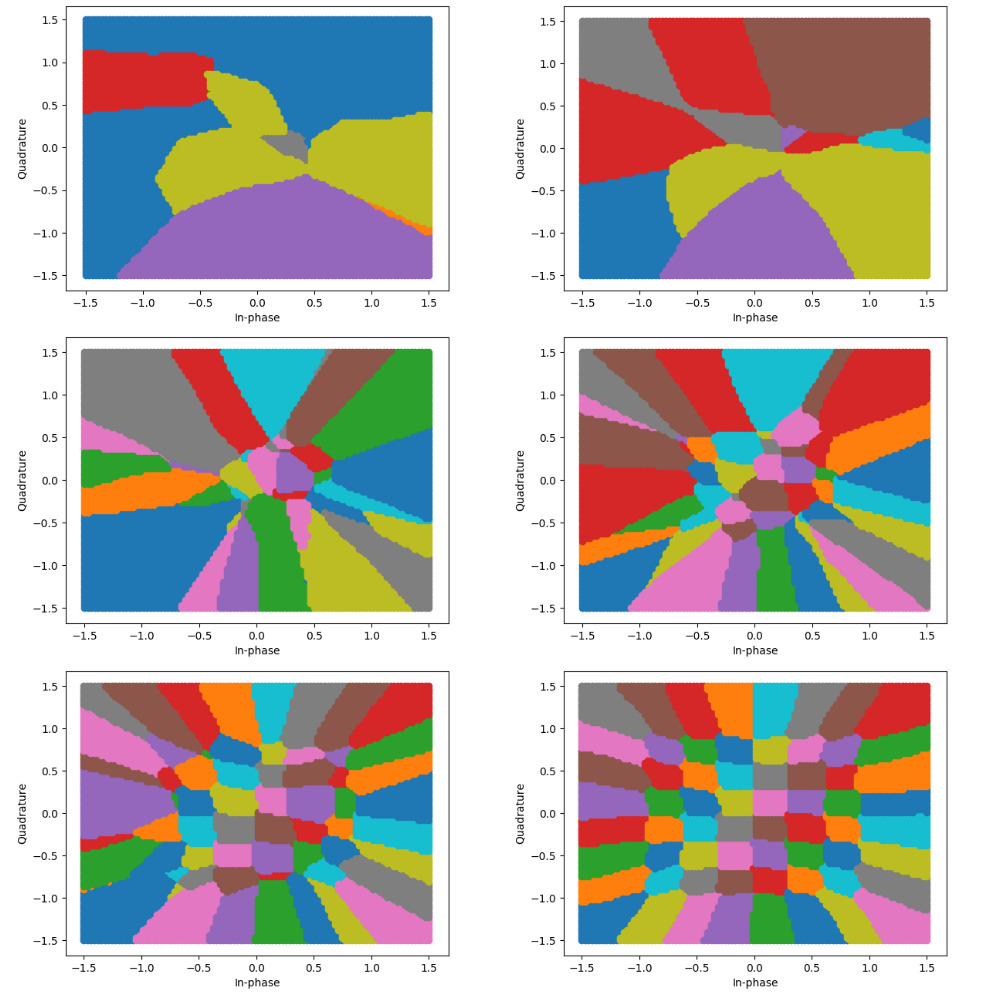
\includegraphics[width=0.9\linewidth]{Thesis/images/linear.jpg}
    \caption{Development of 64-QAM decoder neural network. Upper left after 1 training steps, upper right after 10 training steps, middle left after 300 training steps, middle right after 500 training steps, bottom left after 1000 training steps and bottom right after the last, 24576th training step}
    \label{fig:linear}
\end{figure}

\subsection{Neural network decoder and equalizer}
Decoding signals which are only distorted by Gaussian noise is not a practical example of machine learning in an optical receiver. More of the receiver DSP has to be included in the machine learning algorithm. Because the conventional way of filtering includes a FIR that uses data from the near past, the machine learning network should also include the past data sequence. Therefore, a suitable machine learning network for replacing the entire DSP chain would be to use an RNN-like structure, such as an LSTM.

 In this experiment, the four input nodes of the LSTM are the in-phase and quadrature energy levels of both polarizations. The N output nodes $h_k, k\in\{1..L\}$ are the predicted bit of both polarization, where N is $N = 2\log_2(M)$, in which M is the alphabet size of the modulation. How the weights of the LSTM are trained is depicted schematically in Fig.~\ref{fig:lstm_training}.

\begin{figure}
    \centering
    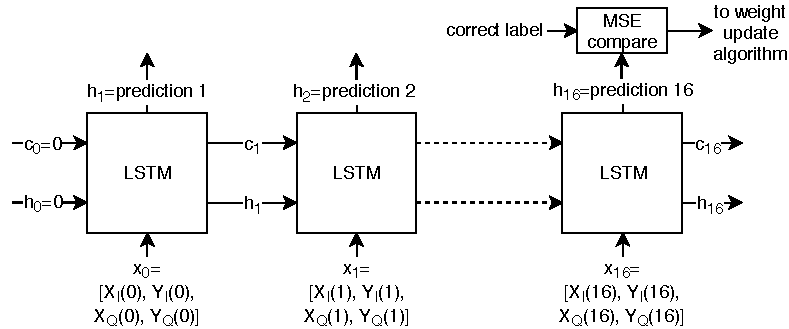
\includegraphics[width=0.9\linewidth]{Thesis/images/lstm_training.pdf}
    \caption{Training of an LSTM, where the sequence length L is 16}
    \label{fig:lstm_training}
\end{figure}

After training, an indefinite discrete sequence of impaired symbol energy levels can be sent through the network. The network gives a prediction for every given input and is no longer dependent on the predefined sequence length $L$.

The parameters of the data and signal impairments are shown in Table~\ref{tab:parameters}. The resulted signal constellation of the original signal is given in the upper left plot in Fig.~\ref{fig:transmitted}. For the X-polarization of this original signal, the first 16 symbols are shown in a 3D time-plot in the upper right plot in Fig.~\ref{fig:transmitted}.

To limit the required bandwidth of the signal, the signal is pulse-shaped with a root raised cosine filter with a roll-off factor $\beta$ of 0.1. After pulse shaping, the signal constellation and time plot are slightly distorted. The resulting signal constellation and X-polarization time plots are shown in respectively the bottom left and right subplots in Fig.~\ref{fig:transmitted}. This signal is sent by the transmitter.

\begin{table}
    \centering
    \caption{Used parameters of generated data}
    \label{tab:parameters}
    \begin{tabular}{c|c}
        Parameter & Value\\
        \hline
        Modulation & QPSK\\
        Amount of symbols per polarization & $2^{20}$\\
        Symbol rate & 25GBd\\
        $\beta$ of RRcos & 0.1\\
        SNR & 15\\
        $\theta$ of PMD & $\frac{\pi}{5}$\\
        $\tau_{DGD}$ of PMD & 40ps\\
        Linewidth of lasers & 1MHz\\
        Frequency offset between lasers & 1MHz\\
    \end{tabular}
\end{table}

\begin{figure}
    \centering
    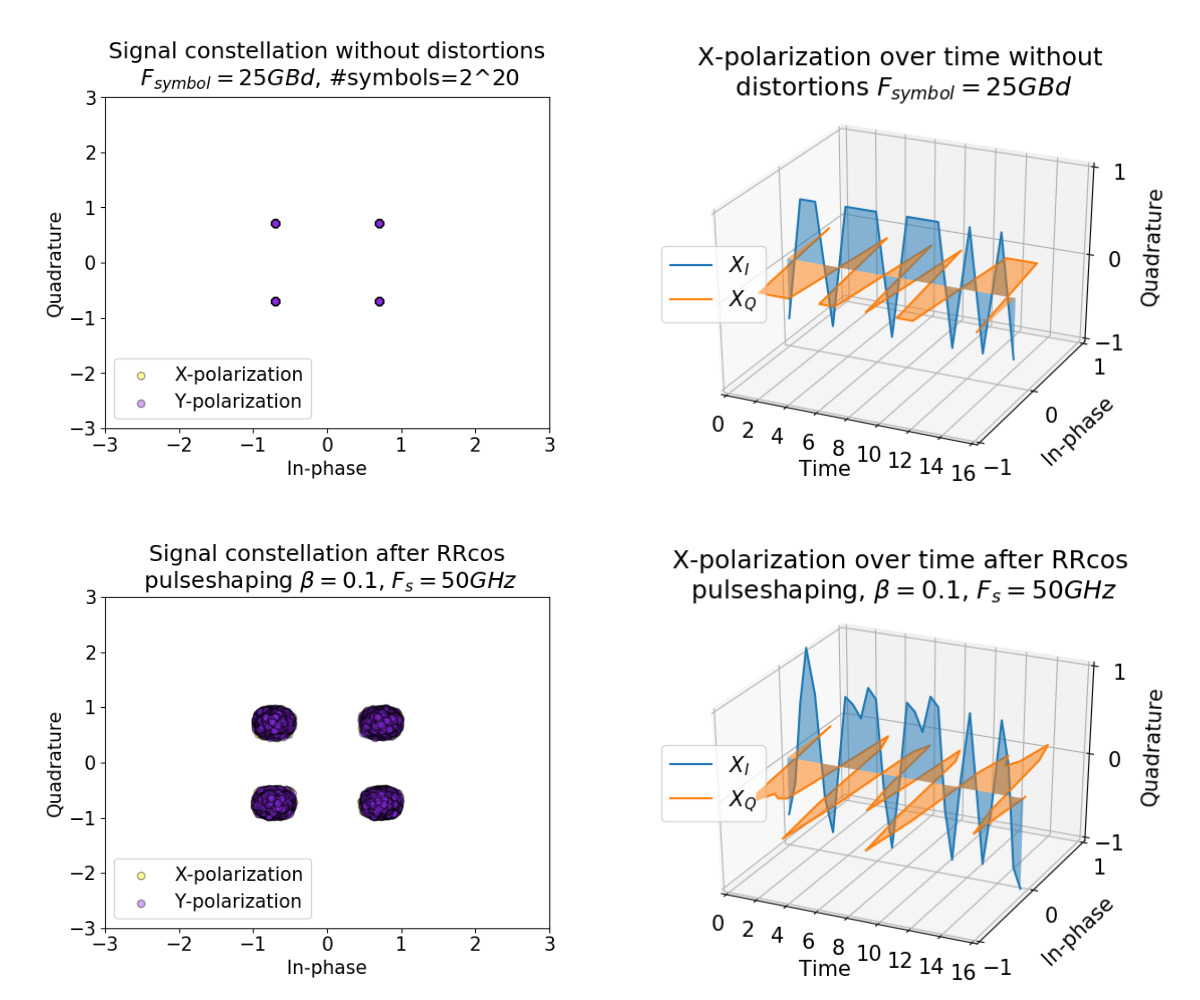
\includegraphics[width=\linewidth]{Thesis/images/transmitted.jpg}
    \caption{Left the signal constellations of the transmitted signal and right the corresponding time plot (in symbol time = 1/25GBd) for the X-polarization. Upper plots are original symbols, bottom plots are pulse-shaped}
    \label{fig:transmitted}
\end{figure}

While transmitting the bandlimited signal, the signal is inevitably impaired by the effects as discussed in section \ref{ch:Medium}. These impairments were artificially added to the transmitted signal. The resulting signal constellation plots for the incrementally added impairments can be seen in Fig.~\ref{fig:impairments}. First, additive Gaussian white noise was added (upper left). Then, PMD impairments were included (upper right). Finally, phase noise (bottom left) and frequency offset (bottom right) were added. This final plot is what the receiver picks up after the ADCs and is input for the recovery neural network.

\begin{figure}
    \centering
    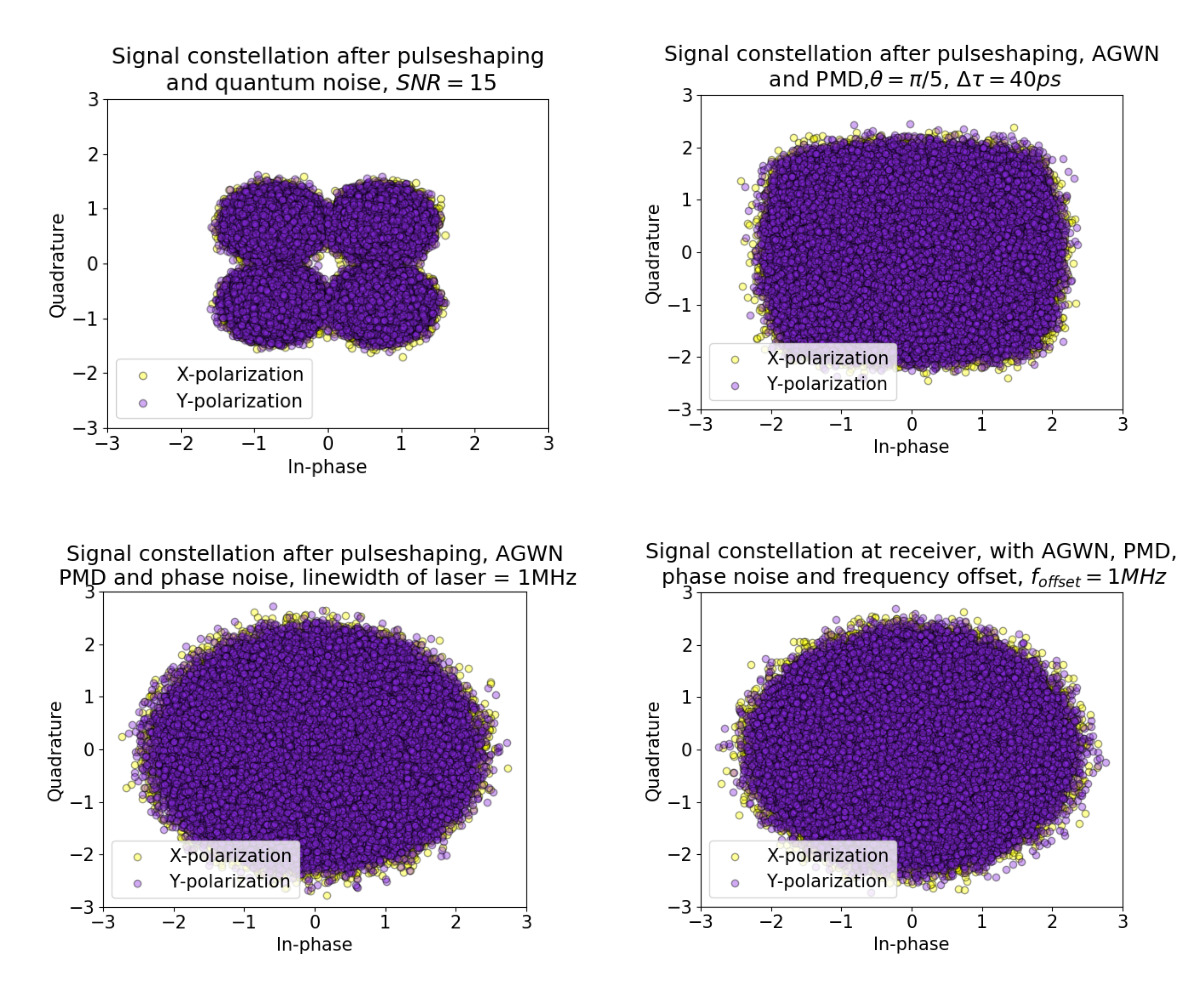
\includegraphics[width=\linewidth]{Thesis/images/impairments.jpg}
    \caption{Signal constellation of received signal, impaired by AGWN (upper left) and PMD (upper right) and phase noise (bottom left) and frequency offset (bottom right)}
    \label{fig:impairments}
\end{figure}

To train the network, the training batches were shuffled to increase the balance of the training data. In this way, the network does not overfit on associated noise of the previous sequence, since this is one of the pitfalls of neural network training.

Unfortunately, the neural network did not show results significantly higher than 50\% (random guessing) after fully training and seemed to have a non-decreasing loss. This is because no carrier phase estimator is input in the network. Therefore, the network could not filter out impairments like phase noise and frequency offset.

To see if the network would have a better performance with extra carrier phase estimation information, the M-th power viterbi-viterbi was added in the network, but without success. Also, single-stage and two-stage blind phase search was added, but no improvement was seen. This is due to the 90 degree symmetric nature of QAM in combination with the shuffling of training data batches. The network can find out what the residue carrier phase offset is (viterbi-viterbi or blind phase search algorithm) within a 90 degree quadrant. However, the network cannot know in which quadrant it is located, because no initial conditions in a randomly selected batch sequence are known. These initial conditions are crucial to predict the integer multiple of 90 degree carrier phase offset of the signal. Thus, prediction acts as a random guess and accuracies cannot by definition have a better performance than 50\%. 

To see if the network would perform without the carrier phase estimator, the phase noise and frequency offset impairments were omitted in the simulation. The substitution of the DSP chain is depicted in Fig.~\ref{fig:dsp} (LSTM). The parameters of the training data and LSTM are given in Table~\ref{tab:lstm}. 

\begin{table}
    \centering
    \caption{Parameters of data and LSTM of simulated experiment}
    \label{tab:lstm}
    \begin{tabular}{c|c}
        Parameter & Value\\
        \hline
        Training sequence length & 16\\
        Learning rate & 0.01\\
        Hidden nodes & 128 (1 layer)\\
        Batch size & 256\\
        Training batches/Testing batches ratio & 90\%/10\%\\
        Loss function & Mean squared error\\
    \end{tabular}
\end{table}

The graphs of the loss functions for the LSTM for various SNRs is given in the upper plot of Fig.~\ref{fig:loss}. The accuracy graphs of the prediction correctness is given in the lower plot of Fig.~\ref{fig:loss}. The final testing data accuracies for the SNR of 30, 15 and 6 were respectively 100\%, 98,5952\% and 83,5871\%. Convergence happens after around 50.000 symbols.

\begin{figure}
    \centering
    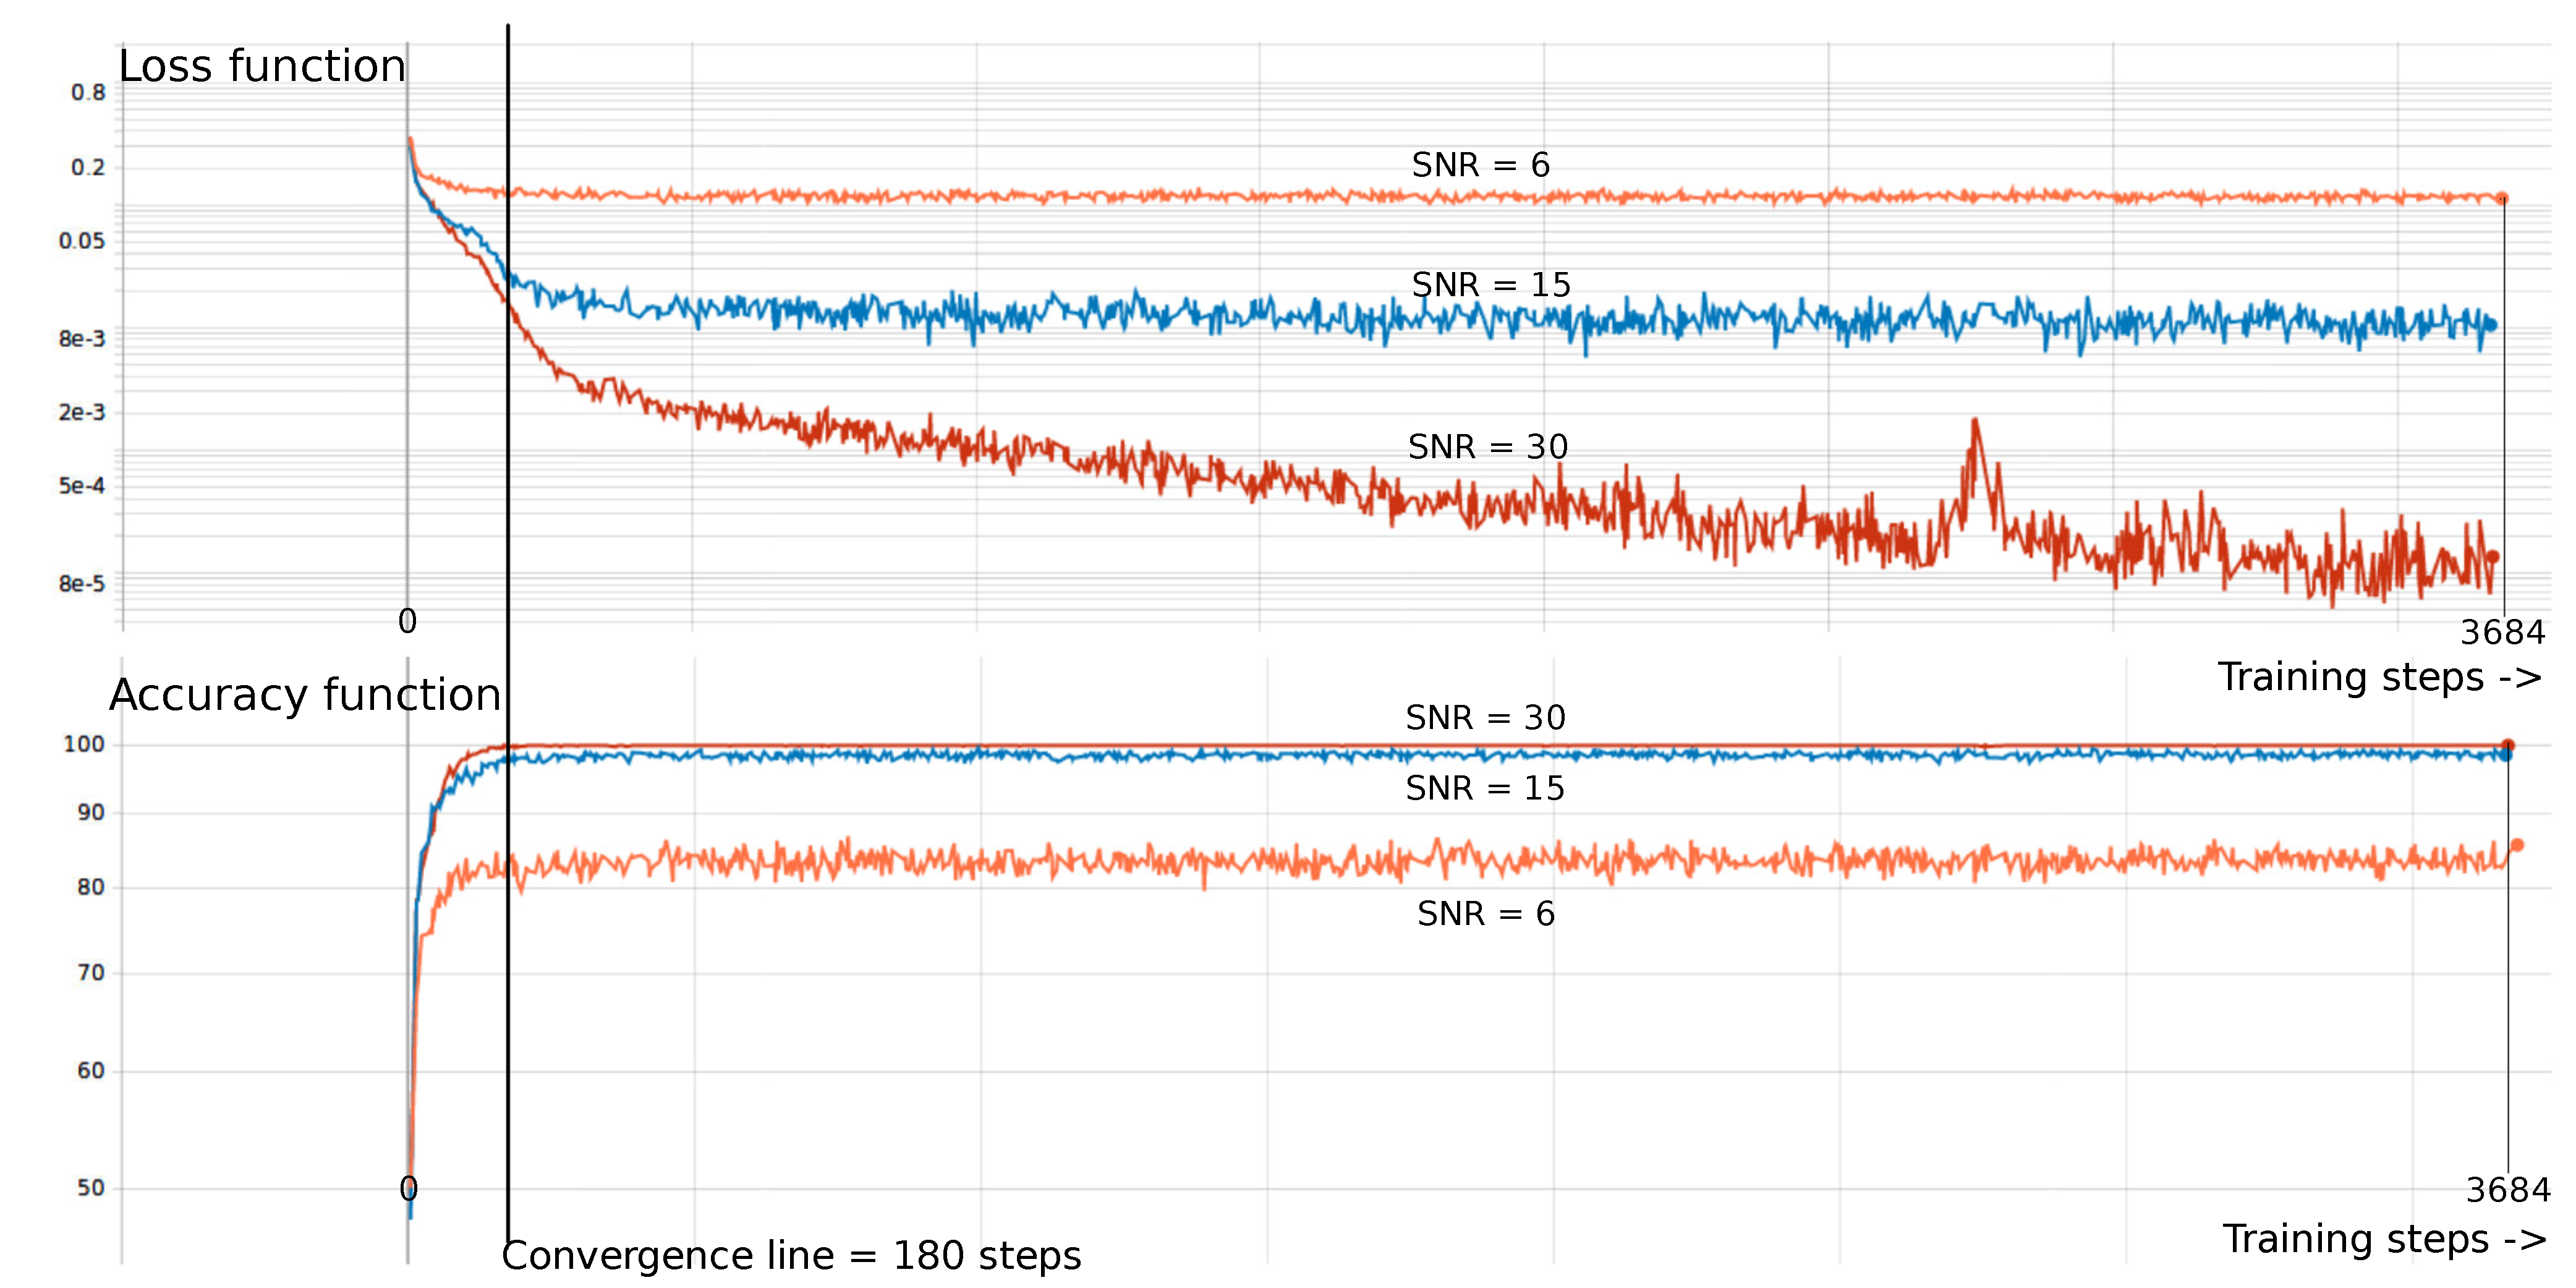
\includegraphics[width=\linewidth]{Thesis/images/loss.pdf}
    \caption{Loss function and accuracy function of LSTM, red curve: SNR 30, blue curve: SNR 15, orange curve: SNR 6. X-axis depicts the amount of training steps. Logaritmic Y-axis.}
    \label{fig:loss}
\end{figure}

\subsection{Real data experiment}
To test the LSTM performance with real data, test data from a optical fiber lab was used. The modulation of this data is 8-QAM. 65536 pseudo-random symbols were sent which are pulse-shaped by a root raised cosine filter with roll-off factor $\beta=0.01$. The data was sent once through a standard single mode optical fiber (SSMF) of 75km and was amplified once by an erbium-doped fiber amplifier (EDFA). The frequency offset was separately compensated for, because the network cannot filter this on its own. In Fig.~\ref{fig:input}, the input constellation can be seen on the left and the output constellation on the right. The parameters of the training data and the LSTM are given in Table~\ref{tab:real_parameters}. The final obtained accuracy of the prediction network is 83.2145\%. However, this data could be detected with no errors with conventional techniques.

\begin{figure}
    \centering
    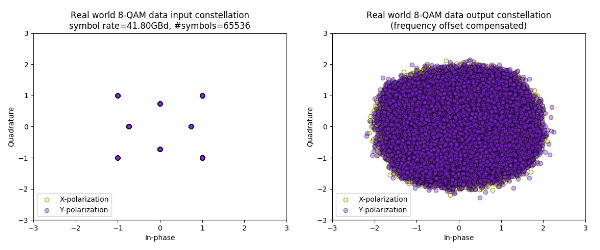
\includegraphics[width=\linewidth]{Thesis/images/real.jpg}
    \caption{Input constellation plot of real world 8-QAM data (left) and output constellation of 8-QAM signal after 75km of SSMF with one EDFA amplification (right)}
    \label{fig:input}
\end{figure}

\begin{table}
    \centering
    \caption{Parameters of data and LSTM of real world experiment}
    \label{tab:real_parameters}
    \begin{tabular}{c|c}
        Parameter & Value\\
        \hline
        Training sequence length & 32\\
        Learning rate & 0.02\\
        Hidden nodes & 256 (1 layer)\\
        Batch size & 128\\
        Training batches/Testing batches ratio & 90\%/10\%\\
        Loss function & Mean squared error\\
    \end{tabular}
\end{table}

\section{Discussion}
The results of the simulated and real data do not show improvement in comparison with the currently deployed DSP chain hardware. The current DSP chain has a BER of several orders of magnitude lower. However, it is difficult to find out what exactly is causing this as intermediate calculations in neural networks do not necessarily have a clear meaning. Furthermore, carrier phase estimation is not included in the LSTM and therefore it cannot properly filter out phase noise and frequency offset.

The are some advantages of a machine learning approach to the optical coherent receiver signal recovery problem over the conventional way. One of these advantages is that it is able to filter both linear and non-linear impairments due to the non-linear Sigmoid activation function embedded in the network. Furthermore, no knowledge is needed about the transmission line and signal impairments do not have to be modeled correctly, as the network will learn how to deal with any kind of impairment, given a training data sequence of a long enough length. Besides that, all the hardware blocks that are in the conventional receiver DSP can be combined into just a single neural network. Adaptive filters can be replaced by a single fixed and static neural network.

New research has to be done to increase the prediction accuracy of the network by monitoring exactly what is happening inside the LSTM and try different specializations of LSTMs to make the network more suitable to the problem. Besides that, it has to be researched how the carrier phase estimator block can be implemented inside the neural network by either a separate network or by increasing the input dimensions of the network with extra information such that the integer multiple of 90 degrees carrier phase can be recovered.

\section{Conclusion}
The conventional optical coherent transmission system was discussed. Machine learning techniques that are suitable to aid the optical coherent receiver were studied. Afterwards, the simulation and real world experiments have shown that the DSP chain can partially be aided with machine learning techniques with regular and recurrent neural networks.

However, for now, these machine learning techniques as a substitute for DSP in optical coherent receivers is not yet feasible. Before this becomes an interesting option, there needs to be more understanding on how to improve the BER of a neural network solution and how the carrier phase estimation can be included in the network.

\balance

\bibliographystyle{IEEEtran}
\bibliography{references}

\end{document} 